\section{Introducción al Sistema de Manejo de Eventos de \nombreFramework}
Uno de los principales objetivos de este proyecto es que una red de Petri esté a
cargo del manejo completo de la concurrencia y el asincronismo de un sistema informático. Para
logralo, se implementó el monitor de petri por software descripto en la
sección \emph{\color{red} CITA REQUERIDA seccion monitor}.
El mismo está basado en la implementación previa realizada en \cite{codegen}.
Este monitor permite delegar la concurrencia y asincronismo del
sistema a una red de Petri. Por ejemplo, fue utilizado con éxito en
\cite{Bentivegna-Ludemann}.

Sin embargo, la utilización directa del monitor es engorrosa y genera un
alto grado de acoplamiento entre el software de usuario y la red de Petri. La
red queda asociada directamente a los eventos del mundo real. La principal
desventaja de tener un sistema acoplado a la red de petri es que disminuye la
escalabilidad del sistema. Esto se debe a que la sustitución de la red (o su modificación) implica
también un cambio en el código del software, dificultando el desarrollo
iterativo de un sistema. Por otro lado, impide la realización de redes
genéricas, más versátiles, útiles para resolver diferentes problemas de las
mismas características.

Otro objetivo del proyecto consiste en la facilidad de uso. Como se explicó
anteriormente, la utilización directa del monitor es complicada y puede
favorecer a la generación de errores, ya que deben crearse todos los hilos de
ejecución y deben programarse los disparos de transición de forma manual en el
código. Ante un cambio en la red de petri deben modificarse todos los disparos
de transición, pudiendo llevar a una incorrecta sincronización de los hilos si
no se realiza con especial precaución.

Finalmente, otro objetivo importante es el de crear una herramienta que permita
al usuario estructurar el proyecto utilizando patrones de diseño de forma
simple. En el caso de utilizar el monitor de forma directa, el diseño del
software queda en manos del usuario desarrollador. Esto significa que la
decisión de utilizar o no patrones de diseño es tomada por el usuario. De
esta forma se desaprovecha la oportunidad de reutilizar ciertos aspectos de
diseño que se consideran pertinentes. Por ejemplo el patrón command descripto en
\cite{chimp}, o algunas caracteristicas similares a un diseño MVC que se pueden
observar en los sistemas sincronizados por Petri. Este último ejemplo se explica
con mayor detalle en la sección \emph{\color{red} CITA REQUERIDA Patrón MVC
en el framework?}.

Como resultado de este análisis, se llegó a la conclusión de que se puede
aprovechar mejor el potencial del monitor si se encuentra embebido en un
framework que se encargue de desacoplar el código de usuario de la lógica de
disparos y de sincronización de hilos. 
Una conclusión de similares características se desprende de
\cite{Bentivegna-Ludemann}, donde los autores expresan: ``La debilidad encontrada en el proceso de elaboración del
software, es que resultó problemático vincular los hilos con las transiciones de
la RdP. Esto se debe a que, en el código de las acciones, quedó embebida la
relación de éstas con las transiciones. Por lo cual, queda en evidencia que es
necesaria la existencia de un framework para automatizar y facilitar la
vinculación entre eventos, acciones y transiciones.''


\section{Red de Petri como procesador de Eventos}
Se puede definir a un sistema desarrollado utilizando el monitor como un
programa de software que intercambia eventos con la red de Petri y con su
entorno físico.

\begin{figure}[h]
	\centering
	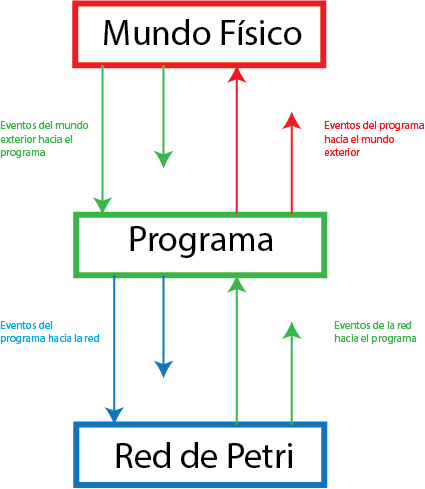
\includegraphics[width=75mm]{eventos_petri-programa-mundo}
	\caption{Intercambio de eventos en un programa sincronizado por Red de Petri}
	\label{fig:eventos_petri-programa-mundo}
\end{figure}

El programa puede acceder a hardware del mundo físico, ya sea para realizar una
acción (por ejemplo utilizando actuadores) o  para obtener eventos del mundo
exterior y comunicarselos a la red de Petri (utilizando sensores, por ejemplo).

La red toma los eventos del mundo exterior y los combina con condiciones del
problema y de sincronización para emitir eventos de salida hacia el programa. La
red es básicamente un procesador de eventos.\cite{chimp}

Este concepto se amplía en la sección Eventos Físicos y Eventos
Lógicos de \cite{chimp}. En esta sección se distingue la existencia de los dos
tipos de eventos mencionados, y se los define como:
  \begin{itemize}
    \item Eventos Lógicos: eventos que son comprensibles por el monitor de
    redes de Petri, y están inherentemente asociados a transiciones de la red
    misma y sus colas.
    \item Eventos Físicos: suceden en el mundo físico y representan sucesos del
    dominio del problema
  \end{itemize}

Tras la incorporación del concepto de eventos lógicos y físicos, los autores
proponen en \cite{chimp} un diagrama de arquitectura de alto nivel como el
siguiente:

\begin{figure}[h]
	\centering
	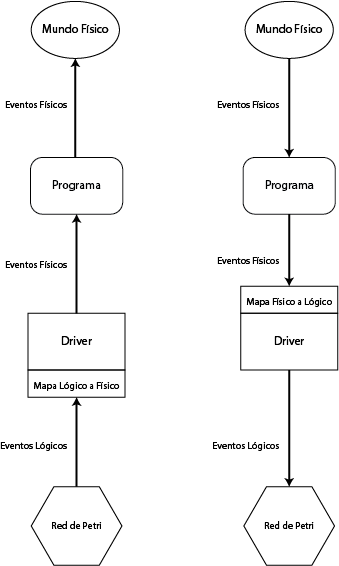
\includegraphics[width=75mm]{eventos_fisicos-logicos}
	\caption{Arquitectura con Eventos Físicos y Lógicos}
	\label{fig:eventos_fisicos-logicos}
\end{figure}





\section{Requerimientos del Sistema de Manejo de Eventos de \nombreFramework}
A continuación se listan los requerimientos establecidos para el nuevo sistema
de manejo de eventos.

\begin{itemize}
  \item 
\end{itemize}



Para explicar el esquema de comunicación de \nombreFramework , primero deben
detallarse otros conceptos inherentes a la misma.


\subsection{Condiciones de Ejecución Síncronas y Asíncronas}
Las condiciones para la ejecución de una acción pueden ser:
  \begin{itemize}
	\item Síncronas: Por ejemplo, condiciones booleanas derivadas del estado del
		sistema que realizan cambios en el flujo de instrucciones del mismo (saltos
		condicionales).
	\item Asíncronas: Por ejemplo, eventos provenientes del mundo exterior o
		señales / mensajes entre hilos / procesos.
  \end{itemize}
  
\subsection{Eventos Lógicos, Programáticos y Físicos}
Los eventos de interés para el sistema pueden ser de tres tipos:
  \begin{itemize}
    \item Eventos Lógicos: eventos que son comprensibles por el monitor de
    redes de Petri, y están inherentemente asociados a transiciones de la red
    misma y sus colas
    \item Eventos del Software: eventos que son comprensibles por el
    subsistema de manejo de eventos y están asociados a acciones del
    software de usuario.
    \item Eventos Físicos: eventos reales que suceden en el mundo físico y
    representan sucesos del dominio del problema. Pueden ser eventos fisicos de
    salida (por ejemplo, al mover un actuador utilizando el programa), o de
    entrada (por ejemplo el cambio de una variable física siendo monitoreada por
    el programa).
  \end{itemize}
  
  
\subsection{Componentes de un sistema desarrollado con \nombreFramework}
Se puede dividir un sistema desarrollado con \nombreFramework en tres partes.
\begin{itemize}
\item Por un lado existe un monitor de redes de Petri, encargado de analizar el
cumplimiento de las condiciones para la ejecución de ciertas partes de código
(acciones). 
\item La segunda parte esta compuesta por un subsistema de manejo de eventos
programáticos, que permite la separación de los eventos lógicos y programáticos
del sistema, la suscripción a dichos eventos programáticos, y la sincronización
y ejecución de las acciones de software suscriptas. El mismo actúa como un
intermediario entre el código del usuario y el monitor de redes de Petri,
permitiendo desacoplar la red de Petri del código de usuario. 
\item Por último, el programa de usuario, que contiene todas las acciones
concretas a realizar, con sus correspondientes suscripciones a eventos
programáticos.
\end{itemize}
  
  
 
La propuesta para lograr el objetivo planteado es un modelo donde el monitor de
red de Petri asume la responsabilidad de verificar las condiciones asíncronas y
de mantener el estado del sistema. De esta forma será la red quien conozca y
analice ese tipo de condiciones.
Los tipos de condiciones que entran bajo consideración del monitor de Petri son:
\begin{itemize}
\item El disparo de eventos provenientes de sistemas externos que llegan en cualquier momento
durante la ejecución y sin ningún orden establecido. Así los estados locales de la red son
mantenidos en causalidad de los procesos que se ejecutan y explicitan los eventos
externos.
\item Condiciones de sincronización que permitan ordenar la realización de tareas en el tiempo.
\item Condiciones impuestas por el dominio del problema. Así la red mantiene su estado en
causalidad de las restricciones del problema.
\end{itemize} \cite{chimp}
\\
Por otro lado, el subsistema manejador de eventos programáticos se encarga de
desacoplar el software del usuario de la red de Petri para relacionar eventos
físicos con eventos lógicos. De esta manera se consigue que las transiciones no
queden asociadas directamente a acciones del programa y, por ende, no se le dé
a la red semántica de un dominio de problema en particular.
Esto trae aparejadas las siguientes ventajas:
  \begin{itemize}
	\item Las redes de Petri se vuelven más genéricas y por lo tanto reutilizables,
    puesto que no hay semántica de un dominio de problema en ellas. Ergo una
    misma red se puede utilizar para resolver problemas diferentes.
	\item El modelo de red de Petri puede cambiar por completo sin afectar al
       programa.
 	Simplemente reconfigurando los mapas de relación de eventos el sistema
 	continúa funcionando
  \end{itemize} \cite{chimp}
\\

 El programa de usuario sólo se limitará a describir las acciones(que pueden
 desencadenar eventos físicos de salida o manejar eventos físicos de entrada)
 y asociarlas a los eventos programáticos que correspondan.
 \\

En este proyecto se utilizan redes de Petri no autónomas. Se dispone de las
etiquetas especificadas en \emph{\color{red} CITA REQUERIDA}. La comunicación
entre el subsistema de manejo de eventos programáticos y el monitor de Petri se
realiza utilizando las interfaces proporcionadas por el monitor.
